\documentclass[../main.tex]{subfiles}

% Aquí se debe describir la forma en la que el grupo se ha coordinado. Además, para cada miembro del grupo se deben indicar las horas totales invertidas en la realización de la práctica, así como un desglose por tarea y una descripción de las tareas realizadas.

\begin{document}

\section{Configuración del kernel}

En este primer apartado se va a comentar cuál es la configuración del kernel de la distribución sobre la que se ha realizado la práctica. 

Los fuentes de Linux se han obtenido del fichero \it{kernel-rt.xz}, que se encuentra en el directorio de prácticas de la asignatura, en el servidor Hendrix \cite{fuentes-Linux}. Sobre ellos ya se ha aplicado el parche tiempo real, por lo que al ejecutar \it{uname -r} en la distribución, el release que aparece es \it{3.8.13-rt14}.

No obstante, durante la configuración previa a la compilación, se eligió uno de los modelos de expulsión que se remarcan en la siguiente imagen:

\begin{figure}[h]
\centering
\includegraphics[width=0.8\textwidth]{imagenes/Apartado0-Kernel-preemtion_model.png}
\caption{Captura del menú de configuración del modelo de expulsión}
\end{figure}

Por lo tanto, si bien el kernel usado tiene el parche tiempo real, el modelo de expulsión no es \it{Full Preemtion}, y por lo tanto no se fuerza a que todas las actividades del kernel sean planificables. Por ese motivo, los tiempos medidos son menores que los que se esperaba obtener, porque desde el \it{irq\_handler} se salta directamente a la \it{ISR}, eliminándose así la latencia de pasar entre medio por el planificador. Sobre el diagrama de las diapositivas de clase \cite{diagrama-latencia}, puede verse de la forma siguiente: 

\begin{figure}[h]
\centering
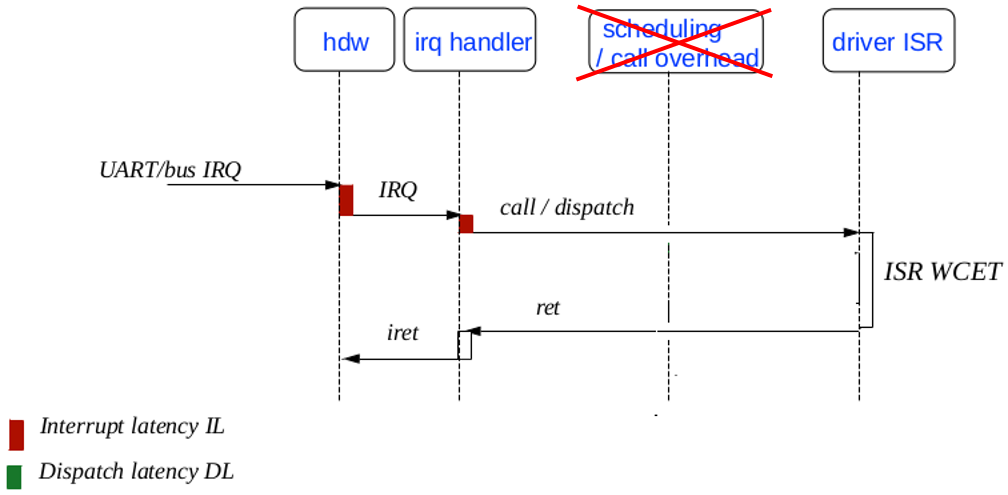
\includegraphics[width=0.7\textwidth]{imagenes/Apartado0-LatenciaInterrupcion.png}
\caption{Diagrama de clase editado para evidenciar que no se pasa por el scheduler}
\end{figure}

\end{document}